\chapter*{Einleitung} \addcontentsline{toc}{chapter}{Einleitung}
\textbf{Definition:\;} Eine \wichtig{Berechnung} ist ein Prozess, der f�r eine beliebige Eingabe aus einem Eingaberaum in endlich vielen elementaren, deterministischen Schritten eine vorher spezifizierte Ausgabe bestimmt. \abstand

\textbf{Beispiel:}
\begin{itemize}
    \item ganze Zahl $\Rightarrow$ Primzahlzerlegung
    \item Graph mit Kantengewichten $\Rightarrow$ MST (minimal aufspannender Baum)
    \item Polynom �ber $\rat$ $\Rightarrow$ Nullstelle
\end{itemize}
\seite%

\textbf{Themen der Vorlesung:}
\begin{itemize}
    \item Modelle f�r Berechnung
    \item Gemeinsamkeiten (Simulation) und Unterschiede
    \item Berechenbarkeit und Endscheidbarkeit
    \item Church'sche These
    \item Komplexit�t einer Berechnung
    \item P-NP-Problem
    \item Kontextfreie Sprachen
    \item Grammatiken und die Chomsky-Hierarchie
\end{itemize}
\pagebreak

\textbf{Beispiel:}
\begin{enumerate}
    \item Entwurf eines endlichen Automaten zur Steuerung einer Ausgangst�r mit Eingangssperre: \par
    \begin{center}
        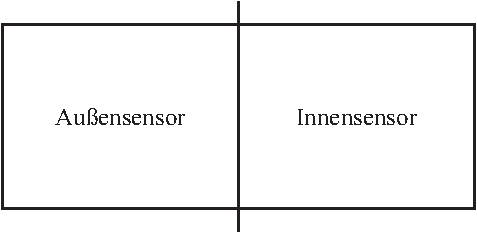
\includegraphics{skript/grafiken/ausgangstuerbild}
    \end{center}
    \begin{tabular}{lccl}
        Eingaben:\; & I & -- & nur Innensensor \\
        & A & -- & nur Au�ensensor \\
        & B & -- & beide \\
        & K & -- & keiner
    \end{tabular}
    \begin{center}
        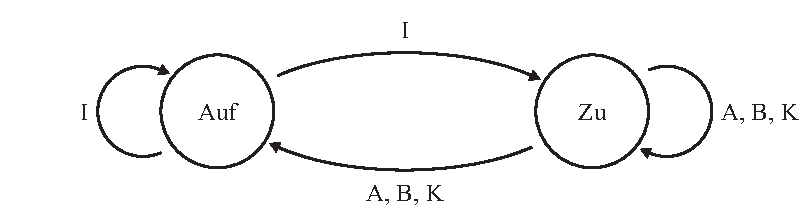
\includegraphics{skript/grafiken/ausgangstuerzustand}
    \end{center}
    \item Postsches Korrespondenzproblem: \\
    Alphabet $\Sigma$ mit den W�rtern $w_1, w_2, \ldots, w_k$ und $v_1, v_2, \ldots, v_k$ \\
    Eingabe: $(w_1, v_2), (w_2, v_2), \ldots (w_k, v_k)$ \\
    Frage: Gibt es eine Indexfolge (mit Wiederholungen) $i_1, i_2, \ldots, i_n$, so dass $w_{i_1} w_{i_2} \ldots w_{i_n} = v_{i_1} v_{i_2} \ldots v_{i_n}$? \\
    Zwei aller m�glichen Eingaben:
    \begin{enumerate}
        \item $\overbrace{(1,101)}^a, \overbrace{(10,00)}^b, \overbrace{(011,11)}^c$ \\
        Indexfolge: $a, c, b, c$ \\
        linke Seite: $1 \; 011 \; 10 \; 011$ \\
        rechte Seite: $101 \; 11 \; 00 \; 11$
        \item $(001,0), (01,011), (01,101), (10,001)$ \\
        k�rzeste L�sung: 66 Paare
    \end{enumerate}
    Dieses Problem ist im Allgemeinen nicht entscheidbar (siehe \ref{entscheidbar})!
\end{enumerate}
\seite
